\documentclass[a4paper,12pt]{article}

\usepackage{header}

\usepackage[pages=all]{background}
\backgroundsetup{
  scale=3.7,
  color=gray,
  opacity=0.15,     
  angle=45,         
  contents={github.com/int28t/hse-se-lecture-notes}
}

\title{Семинары по дискретной математике (1 курс, 25-26)}
\author{github.com/int28t/hse-se-lecture-notes}
\date{}

\begin{document}
    \pagestyle{empty}
	\maketitle
    \begin{flushright}
		Хрыстик Михаил Андреевич
	\end{flushright}
	\tableofcontents{}
    \newpage
    \pagestyle{plain}
    \input{./lectures/lecture notes_01_[20.11.2025].tex}
    \newpage
    \input{./lectures/semx1.tex}
    \newpage
    \input{./lectures/semx2.tex}
    \newpage
    \section{Комбинаторика}

\begin{definition}
    Число сочетаний --- количество способов выбрать $k$-элементное подмножество из $n$-элементного множества. Обозначается $C^k_n$ или $\binom{n}{k}$.
\end{definition}

\[
    C^k_n = \frac{n!}{k!(n-k)!} \ (n!=1\cdot 2 \cdot 3 \cdot \ldots \cdot n, 0!=1)
\]

\subsection{Задача 13}

\begin{figure}[H]
  \centering
  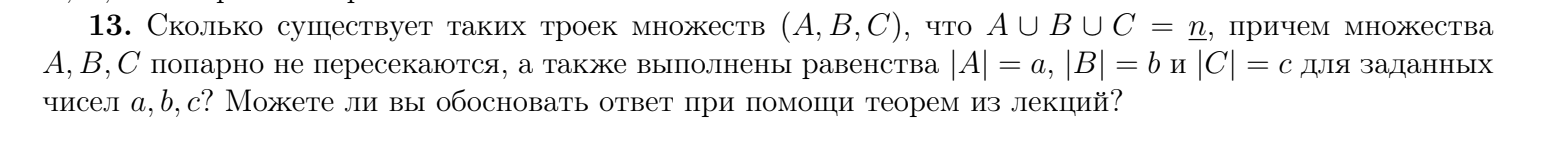
\includegraphics[width=1\textwidth]{lectures/files/task9-13.png}
  \label{fig:task9-13.png}
\end{figure}

\begin{solution}
    Заметим, что $a + b + c = n$

    \[
        0\ 1\ 2\ 3\ \ldots\ n - 1
    \]

    Выбрать элементы множества $A$ --- $C^a_n$ способов, выбрать элементы множества $B$ --- $C^b_{n-a}$ способов, выбрать элементы множества $C$ --- $C^c_{n-a-b}$ способов. Заметим, что $C^c_{n-a-b} = 1$, так как из оставшихся элементов нужно выбрать все.
\end{solution}

\begin{solution}[Ответ]
    \[
        C^a_n \cdot C^b_{n-a}
    \]
\end{solution}

\subsection{Задача 17}

\begin{figure}[H]
  \centering
  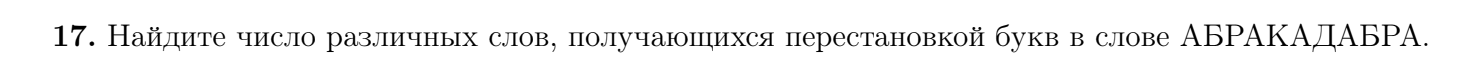
\includegraphics[width=1\textwidth]{lectures/files/task9-17.png}
  \label{fig:task9-17.png}
\end{figure}

\begin{solution}[Ответ]
    \[
        \frac{11!}{2!\ 2!\ 5!}
    \]
\end{solution}

\subsection{Задача 18}

\begin{figure}[H]
  \centering
  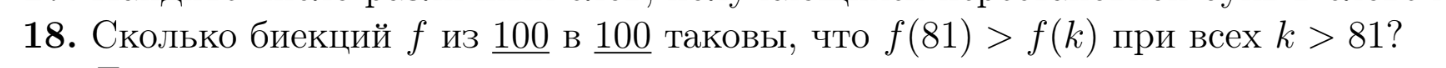
\includegraphics[width=1\textwidth]{lectures/files/task9-18.png}
  \label{fig:task9-18.png}
\end{figure}

\begin{solution}

\[
    f(81) = 18 : 18! \cdot 81!
\]
\[
    f(81) = 19 : 19 \cdot 18 \cdot 17 \cdot \ldots \cdot 2 = \frac{19!}{1!} \cdot 81!
\]
\[
    f(81) = 20 : 20 \cdot 19 \cdot \ldots \cdot 3 = \frac{20!}{2!} \cdot 81!
\]
\[
    \vdots
\]
\[
    f(81) = 99 : 99 \cdot \ldots \cdot 82 \equiv \frac{99!}{81!} \cdot 81!
\]

\end{solution}

\begin{solution}[Ответ]
    \[
        81! \cdot \Sum{k=18}{99} \frac{k!}{(k-18)!}
    \]
\end{solution}

\subsection{Задача 19}

\begin{figure}[H]
  \centering
  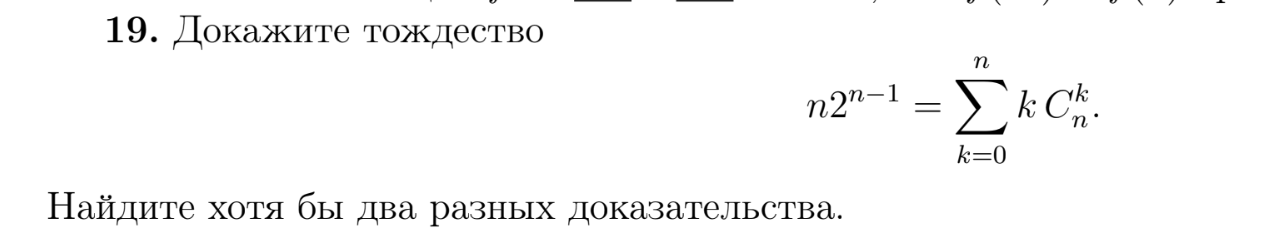
\includegraphics[width=1\textwidth]{lectures/files/task9-19.png}
  \label{fig:task9-19.png}
\end{figure}

\subsubsection{Способ 1. Аналитический}

\begin{solution}
    \[
        (1 + x)^n = 1 \cdot C^0_n + x C^1_n + x^2 C^2_{n} + \ldots + x^n C^n_n 
    \]

    Возьмем производную:
    \[
        n(1 + x)^{n-1} = C^{1}_n + 2x C^2_n + 3x^2 C^3_n + \ldots + n x^{n-1} C^n_n 
    \]
    Подставим $x = 1$:
    \[
        n \cdot 2^{n-1} = \Sum{k = 1}{n} k C^k_n = \Sum{k = 0}{n} k C^k_n
    \]
\end{solution}

\subsubsection{Способ 2. Комбинаторный}

\begin{solution}
    Найдем количество способов выбрать из $n$ человек команду (с произвольным числом участников) и капитана в ней.

    $n$ способов выбрать капитана, $2^{n-1}$ способ выбрать остальных участников команды (каждый может быть либо в команде, либо нет). С другой стороны, $k C^k_n$ --- количество способов выбрать команду из $k$ человек и капитана в ней. Приравнивая эти выражения, получаем искомое равенство.
\end{solution}

\subsubsection{Способ 3. Алгебраический}

\begin{solution}
    \[
        k \cdot C^k_n = \frac{n! k}{k! (n-k)!} = \frac{n (n-1)!}{(k-1)! ((n-1) - (k-1))!} = n \cdot C^{k-1}_{n-1}
    \]
    \[
        2^n = \Sum{k=0}{n} C^k_n
    \]
    \[
        \Sum{k=0}{n} k C_n^k = \Sum{k=1}{n} k C_n^k = n \Sum{k=1}{n} C^{k-1}_{n-1} \overset{m = k - 1}{=} n \Sum{m=0}{n-1} C^m_{n-1} = n \cdot 2^{n-1}
    \]
\end{solution}

\subsection{Задача 20}
\begin{figure}[H]
  \centering
  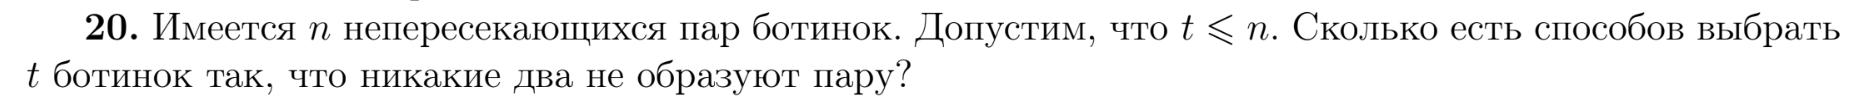
\includegraphics[width=1\textwidth]{lectures/files/task9-20.png}
  \label{fig:task9-20.png}
\end{figure}

\begin{solution}[Способ 1]
    \[
        \frac{2n \cdot (2n - 2) \cdot (2n - 4) \cdot \ldots \cdot (2n - 2(t-1))}{t!}
    \]
\end{solution}

\begin{solution}[Способ 2]
    \[
        C^t_n \cdot 2^t \text{ --- выбор $t$ пар и их расположение}
    \]
\end{solution}

\subsection{Задача 21}
\begin{figure}[H]
  \centering
  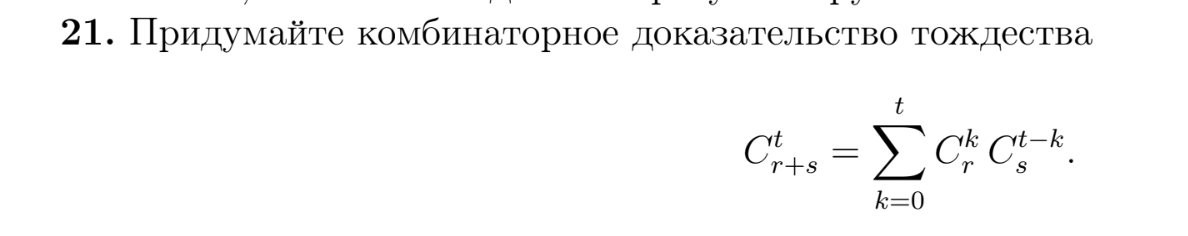
\includegraphics[width=1\textwidth]{lectures/files/task9-21.png}
  \label{fig:task9-21.png}
\end{figure}

\begin{solution}
    Придумаем условие в терминах команд. Пусть есть $r$ мальчиков и $s$ девочек. Сколько способов выбрать среди них команду из $t$ человек?

    По определению $C^t_{r+s}$. В правой части случаи непересекаются, так как отличаются разным количеством мальчиков в команде. Тогда разобьем на случаи по количеству мальчиков в команде. Пусть в команде $k$ мальчиков, тогда $t - k$ девочек. Число способов выбрать таких команд --- $C^k_r \cdot C^{t-k}_s$. Сложив по всем возможным $k$, получаем искомое равенство.
\end{solution}

\subsection{Задача 22}
\begin{figure}[H]
  \centering
  
\includegraphics[width=1\textwidth]{lectures/files/task9-22.png}
  \label{fig:task9-22.png}
\end{figure}

\begin{solution}
    \[
        C^0_n \cdot C^0_n + C^1_n \cdot C^1_n + \ldots + C^n_n \cdot C^n_n = [C^k_n = C^{n-k}_n] = C^0_n \cdot C^n_n + C^1_n \cdot C^{n-1}_n + \ldots + C^n_n \cdot C^0_n =
    \]
    \[
        = [N 21 r=s=t=n] = 2^n
    \]
\end{solution}

\end{document}
